\section{Materiais}
Esta seção descreve os elementos essenciais que viabilizam a condução da pesquisa, contemplando fontes de dados, ferramentas de software e plataformas de hardware utilizadas nas etapas de modelagem, simulação e avaliação do sistema. Esses materiais fornecem o suporte técnico necessário tanto para a construção da base experimental quanto para a execução dos métodos de desenvolvimento e validação apresentados nas subseções seguintes.
\subsection{Base de Dados}

A formação da base de dados é fundamental para o desenvolvimento e validação dos modelos de aprendizado de máquina aplicados à detecção de cavitação. Nesta pesquisa são utilizadas três fontes complementares, abrangendo diferentes contextos experimentais:

\begin{itemize}
	\item \textbf{Falhas em Rolamentos — Case Western Reserve University (CWRU):}  
	Conjunto amplamente utilizado na literatura de diagnóstico de falhas, contendo sinais vibracionais sob diferentes cargas e níveis de dano.  
	\textit{Disponível em:} \url{https://engineering.case.edu/bearingdatacenter/download-data-file}
	
	\item \textbf{Cavitação em Bombas — UWA System Health Lab:}  
	Base pertencente à \textit{Prognostics Data Library}, contendo sinais acústicos registrados em condições controladas de cavitação.  
	\textit{Disponível em:} \url{https://systemhealthlab.com/research-tools/prognostics-data-library}
	
	\item \textbf{Bancada Experimental — Projeto MOMEA (Itaipu Binacional / ParqueTec):}  
	Conjunto experimental obtido com o sistema MomeaProbe/MomeaCapture, utilizado para registrar sinais reais de Emissão Acústica (EA) e vibração em motobombas instrumentadas.
\end{itemize}

A combinação dessas três bases — pública, controlada e experimental — permite avaliar a robustez do modelo em cenários realistas e com diferentes níveis de ruído.

\subsection{Softwares e Ferramentas}

O desenvolvimento desta pesquisa integra um conjunto de ferramentas de software e hardware voltadas à síntese, simulação e avaliação de modelos em FPGA:

\begin{itemize}
	\item \textbf{FINN Framework (AMD/Xilinx):}  
	Utilizado para converter modelos quantizados (QONNX/Brevitas) em arquiteturas \textit{dataflow} otimizadas para FPGA, com geração automática de IPs em HLS/RTL.
	
	\item \textbf{PyTorch e Brevitas:}  
	Empregados no treinamento e quantização das CNNs 1D.
	
	\item \textbf{Vivado Design Suite:}  
	Ambiente para síntese lógica, análise de temporização e geração do \textit{bitstream}.
	
	\item \textbf{Ferramentas do Projeto MOMEA:}  
	Incluem a aplicação MomeaCapture (C++/Qt), rotinas de FFT e algoritmos de compressão e armazenamento via SQLite.
\end{itemize}

\section{Metodologia}

A metodologia foi estruturada com base no modelo de \textit{Descoberta de Conhecimento em Bancos de Dados} (DCBD), proposto por Fayyad, Piatetsky-Shapiro e Smyth (1996). Esse modelo foi adaptado ao contexto de monitoramento por Emissão Acústica (EA), estruturando o pipeline em quatro etapas:

\begin{itemize}
	\item \textbf{Seleção:} coleta e organização dos sinais experimentais;
	\item \textbf{Transformação:} filtragem, segmentação e normalização;
	\item \textbf{Mineração:} aplicação de CNN-1D para detecção de cavitação;
	\item \textbf{Interpretação:} análise dos resultados e extração de conhecimento.
\end{itemize}

Para fins de clareza metodológica, o trabalho foi dividido em duas frentes complementares:  
\textbf{(i) métodos de desenvolvimento} e \textbf{(ii) métodos de avaliação}.

\subsection{Métodos de Desenvolvimento}

Os métodos de desenvolvimento abrangem o ciclo completo de preparação dos dados, modelagem, treinamento e simulação do modelo em FPGA:

\begin{enumerate}
	\item \textbf{Aquisição e Pré-processamento:}  
	Construção da base de dados, remoção de trechos inválidos, normalização e segmentação temporal.
	
	\item \textbf{Modelagem e Treinamento da CNN-1D:}  
	Definição da arquitetura convolucional, escolha de funções de ativação e treinamento com métricas supervisionadas.
	
	\item \textbf{Quantização e Exportação (Brevitas/QONNX):}  
	Aplicação de \textit{quantization-aware training} e conversão do modelo para formato compatível com o FINN.
	
	\item \textbf{Síntese Experimental com o FINN:}  
	Geração do pipeline \textit{dataflow}, simulação de latência, uso de recursos e validação funcional.
\end{enumerate}

\subsection{Métodos de Avaliação}

A avaliação foi conduzida em dois níveis complementares:

\begin{itemize}
	\item \textbf{Avaliação Funcional da CNN-1D:}  
	Acurácia, precisão, sensibilidade, especificidade e matriz de confusão.
	
	\item \textbf{Avaliação da Implementação FPGA (simulada):}  
	Estimativa de uso de recursos (LUTs, BRAMs, DSPs), frequência máxima, latência e throughput, considerando o modelo quantizado.
\end{itemize}

Esses métodos permitem correlacionar diretamente o desempenho do algoritmo com sua viabilidade prática como sistema embarcado.


\subsection{Simulador}

Como a implementação física não será realizada neste projeto, utiliza-se um simulador baseado no FINN e no Vivado. Esse ambiente:

\begin{itemize}
	\item reproduz o fluxo \textit{dataflow} do acelerador;
	\item estima latência, paralelismo e uso de recursos;
	\item simula a inferência em ponto fixo para avaliar o impacto da quantização.
\end{itemize}

Esse recurso permite validar antecipadamente o comportamento do sistema embarcado antes da implementação física.

Figura~\ref{fig:fluxograma_geral} ilustra o fluxo metodológico completo — desde o treinamento offline até a simulação do pipeline embarcado — integrando as etapas de pré-processamento, quantização, compilação e execução no FPGA.

\begin{figure}[H]
	\centering
	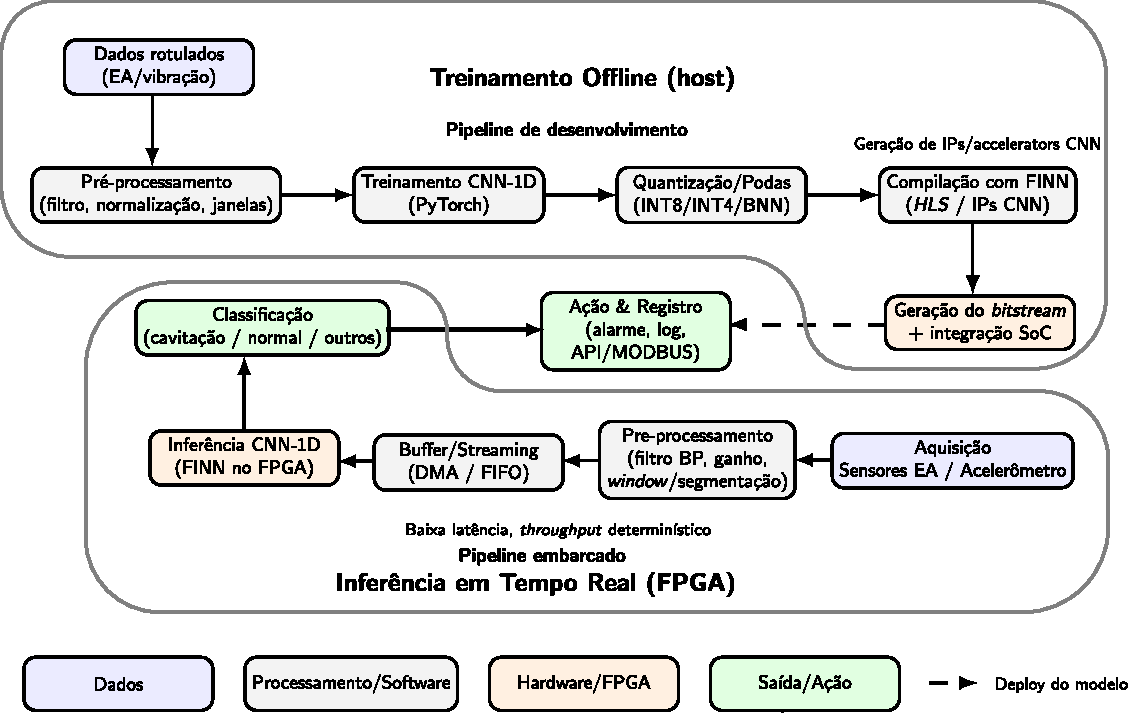
\includegraphics[width=0.95\linewidth]{figs/Fluxograma_Objetivo.pdf}
	\caption{Fluxograma geral dos objetivos do projeto, contemplando as etapas de desenvolvimento e inferência da CNN-1D em FPGA.}
	\label{fig:fluxograma_geral}
\end{figure}

Durante o desenvolvimento, pretende-se definir métricas quantitativas — como latência de inferência, consumo energético e taxa de detecção — que servirão como valores-alvo para a viabilidade prática do sistema embarcado.

